\documentclass[red]{beamer}
\setbeamertemplate{navigation symbols}{}
\usepackage[utf8x]{inputenc}
\usepackage{graphicx}
\usepackage{beamerthemeshadow}

\usetheme{CambridgeUS}
\setbeamercolor{itemize item}{fg=red} % all frames will have red bullets

\begin{document}
\title{Solving CAPTCHAs}
\author[MM, LM, SN, AS]{Mihai Maruseac, Lucian Mogoșanu, Sofia Neață, Adrian Șendroiu}
\date{March 2012}

\pgfdeclareimage{q}{img/q}

\maketitle

\begin{frame}{Admin}
  \begin{itemize}
    \item Team: UnCAPTCHA
      \begin{itemize}
        \item Mihai Maruseac
        \item Lucian Mogoșanu
        \item Sofia Neață
        \item Adrian Șendroiu
      \end{itemize}
    \item Repo: \url{https://github.com/mihaimaruseac/ssl}
  \end{itemize}
\end{frame}

\begin{frame}{Architecture - Overview}
	\begin{center}
	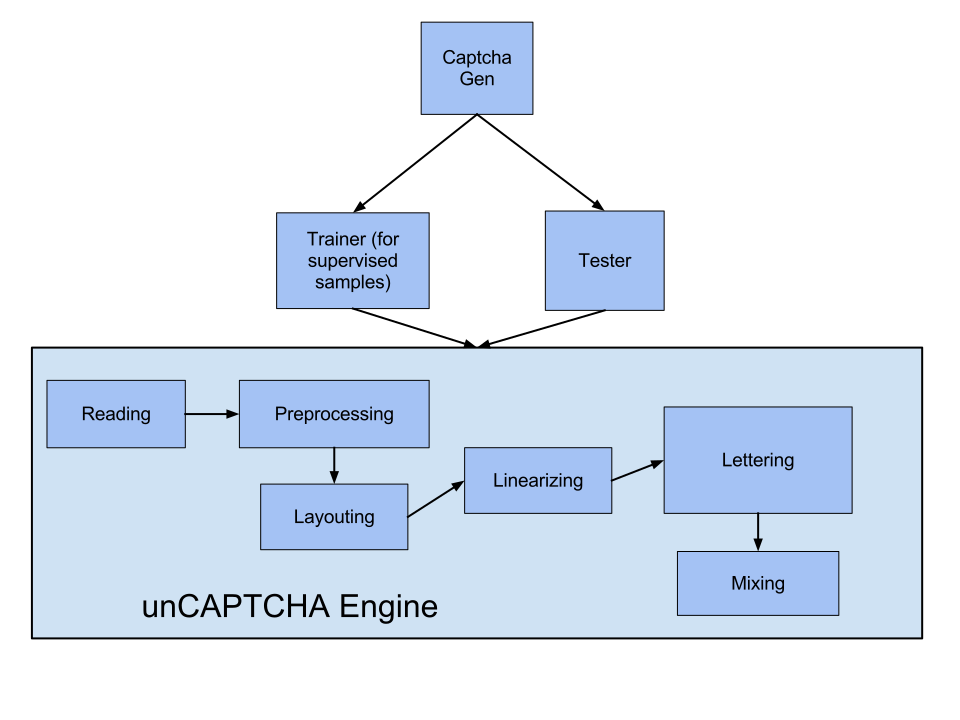
\includegraphics[width=0.85\textwidth]{img/unCAPTCHAarchitecturedraft.pdf}
	\end{center}
\end{frame}

\begin{frame}{Architecture - Overview}
  \begin{itemize}
  	\item Use Securimage to generate CAPTCHAs
	\item Feed them to a trainer and/or a tester
	\item Actual work done by the unCAPTCHA engine
	\begin{itemize}
		\item Pipelined architecture
		\item Easily extensible
	\end{itemize}
  \end{itemize}
\end{frame}

\begin{frame}{unCAPTCHA engine - Reading}
  \begin{itemize}
    \item PNG, PPM, JPEG, BMP
    \item One single internal format
    \item Easier for next stages
  \end{itemize}
\end{frame}

\begin{frame}{unCAPTCHA engine - Preprocessing}
  \begin{itemize}
    \item transform the image
    \item filters
    \item perspective corrections, contrast enhancements
    \item reduce distortions
    \item much clearer image
    \item not a complete preprocessing, needs more data from next stages
  \end{itemize}
\end{frame}

\begin{frame}{unCAPTCHA engine - Layouting \& Linearizing}
  \begin{itemize}
    \item main direction of text, distance between letters, size of letters
    \item separate each letter from the neighbours
    \item achieve near to 0 distortions
  \end{itemize}
\end{frame}

\begin{frame}{unCAPTCHA engine - Lettering \& Mixing}
  \begin{itemize}
    \item guess letter values
    \item most probable letter or a vector of pairs (letter, confidence)
    \item mix letters to form text behind captcha
  \end{itemize}
\end{frame}

\begin{frame}{unCAPTCHA engine - Supervised learning}
  \begin{itemize}
    \item on top of the pipeline
    \item create distorted images and feed them to the engine
    \item testing and parameter tweaking
  \end{itemize}
\end{frame}

\begin{frame}{unCAPTCHA engine - Modifiable pipeline}
  \begin{itemize}
    \item multiple modules
    \item read configuration file and instantiate them
    \item not in beta version
  \end{itemize}
\end{frame}

\begin{frame}{Thank you}
  \begin{center}
    \pgfuseimage{q}
  \end{center}
\end{frame}

\end{document}
